\documentclass[12pt,aspectratio=169]{beamer}
\usecolortheme{udec}
\usetheme{udec}
\usepackage{graphicx}
\graphicspath{{img/},{slides/}}
\usepackage{pgffor}
\usepackage{tikz}
\usepackage{fontspec}
\usepackage{gelasio}
\usefonttheme{serif}
\setmainfont{Gelasio}
\usepackage{polyglossia}
\setmainlanguage{spanish}
% \setbeameroption{show notes on second screen=bottom}

\newcommand<>{\fullsizegraphic}[1]{
	\begin{tikzpicture}[remember picture,overlay]
	\node[at=(current page.center)] {
		\includegraphics{#1}
	};
	\end{tikzpicture}
}

\usepackage{listings}
\usepackage{xcolor}
\definecolor{codegreen}{rgb}{0,0.6,0}
\definecolor{codegray}{rgb}{0.5,0.5,0.5}
\definecolor{codepurple}{rgb}{0.58,0,0.82}
\definecolor{backcolour}{rgb}{0.95,0.95,0.92}
\lstdefinestyle{mystyle}{
    backgroundcolor=\color{backcolour},   
    commentstyle=\color{codegreen},
    keywordstyle=\color{magenta},
    numberstyle=\tiny\color{codegray},
    stringstyle=\color{codepurple},
    basicstyle=\ttfamily\footnotesize,
    breakatwhitespace=false,         
    breaklines=true,                 
    captionpos=b,                    
    keepspaces=true,                 
    numbers=left,                    
    numbersep=5pt,                  
    showspaces=false,                
    showstringspaces=false,
    showtabs=false,                  
    tabsize=2
}
\lstset{style=mystyle}
\usepackage{dirtytalk}

\title{Implementación de una arquitectura para validación de controladores de aeronaves de ala fija en X-Plane}
\subtitle{Memoria de título}
\author{Por Germán Quijada}
\institute{Profesor guía:\\Bernardo Hernández}

\begin{document}
\begin{frame}[noframenumbering]
    \maketitle
\end{frame}

\begin{frame}{Contenidos}
    \tableofcontents
\end{frame}

%% Introducción
\section{Definición de la problematica}

\subsection{Contexto}

\begin{frame}{Contexto}
    \begin{columns}
        \begin{column}{0.45\textwidth}{
                \begin{figure}[t]
                    \centering
                    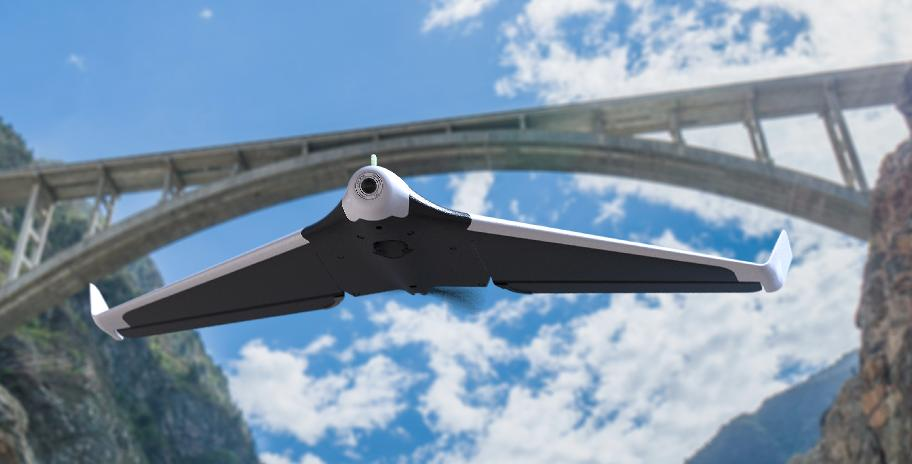
\includegraphics[width=0.9\textwidth]{img/disco-flying.jpg}
                    \caption{Aeronave ``Flying-Disco''}
                \end{figure}
            }
        \end{column}
        \begin{column}{0.45\textwidth}{
                \begin{figure}[t]
                    \centering
                    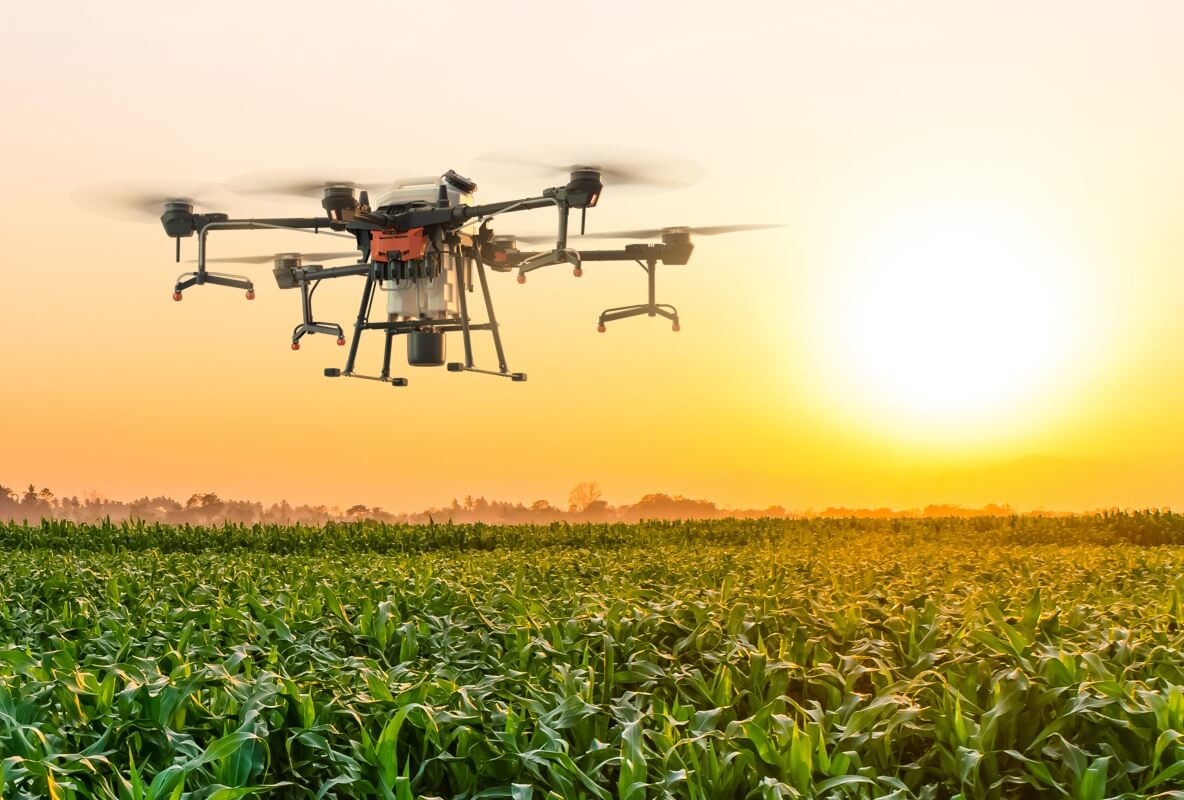
\includegraphics[width=0.9\textwidth]{img/dji-agricola.jpg}
                    \caption{Dron ``DJI''}
                \end{figure}
            }
        \end{column}
    \end{columns}
\end{frame}

\begin{frame}{Concepto}
    Los software controlador de RPAS que utiliza un autopiloto utilizan controladores PID\\
    \pause
    Existen más tipos de controlador que los PID, no implementados en el software actual.
\end{frame}

\begin{frame}{Controladores}
    [pid]
\end{frame}

\begin{frame}{Controladores}
    [otros controladores]
\end{frame}

\subsection{Objetivos}

\begin{frame}{Objetivo}
    Implementación de una arquitectura para validación de nuevos algoritmos de control en microcontroladores para aeronaves de ala fija por medio de la técnica \emph{Processor-in-Loop} con X-Plane.\\
    \vspace{1cm}
    \pause
    \footnotesize{
        \textbf{Objetivos específicos}\\
        \textbf{1.} Estudio de algoritmos de control y opciones de personalización disponibles para estos en los software de autopiloto actuales y selección de software autopiloto base.\\
        \textbf{2.} Desarrollo de extensión de protocolo de comunicación de X-Plane para controladores autopiloto.\\
        \textbf{3.} Implementación de distintos algoritmos de control a los ya implementados en el software y validación en simulador X-Plane como prototipo de arquitectura.\\
        \textbf{4.} Establecer y documentar proceso sistemático para la implementación de algoritmos de control en la nueva arquitectura.\\
    }

\end{frame}

\subsection{Estructura del proyecto}

\begin{frame}{Estructura del proyecto}
    \begin{columns}
        \begin{column}{0.45\textwidth}{
                \centering
                Entorno de desarrollo
            }
        \end{column}
        \begin{column}{0.45\textwidth}{
                \centering
                Diseño de algoritmos de control
            }
        \end{column}
    \end{columns}
\end{frame}

\section{Entorno de desarrollo}

\begin{frame}[noframenumbering]
    \sectionpage
\end{frame}

\begin{frame}{Objetivos}
    \begin{itemize}
        \item
    \end{itemize}
\end{frame}

\begin{frame}{Selección de autopiloto}
    \centering
    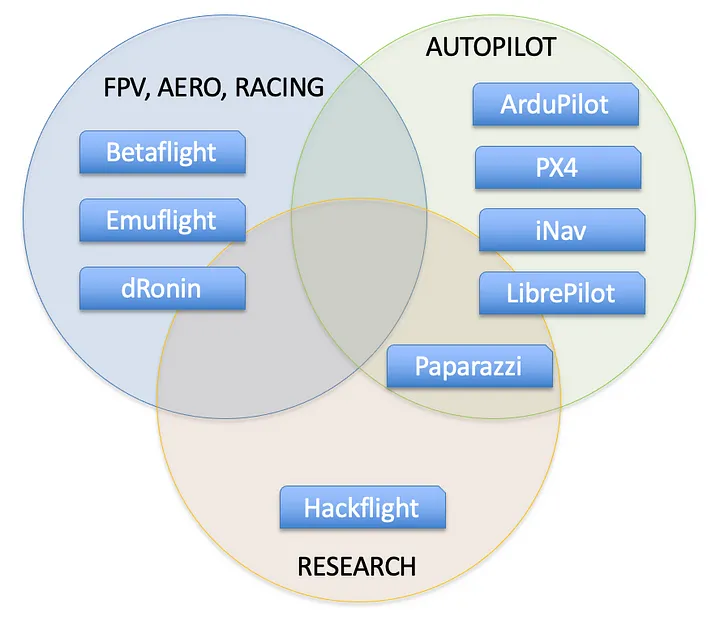
\includegraphics[height=0.8\textheight]{img/opensource-autopilots.png}
\end{frame}

\section{Diseño de algoritmos de control}

\begin{frame}[noframenumbering]
    \sectionpage
\end{frame}

\end{document}